% ch2p21_006: Upgrade to Karl's activity
\documentclass[tikz, border=10pt]{standalone}

\usepackage{tikz}
\usetikzlibrary{intersections}

\begin{document}
	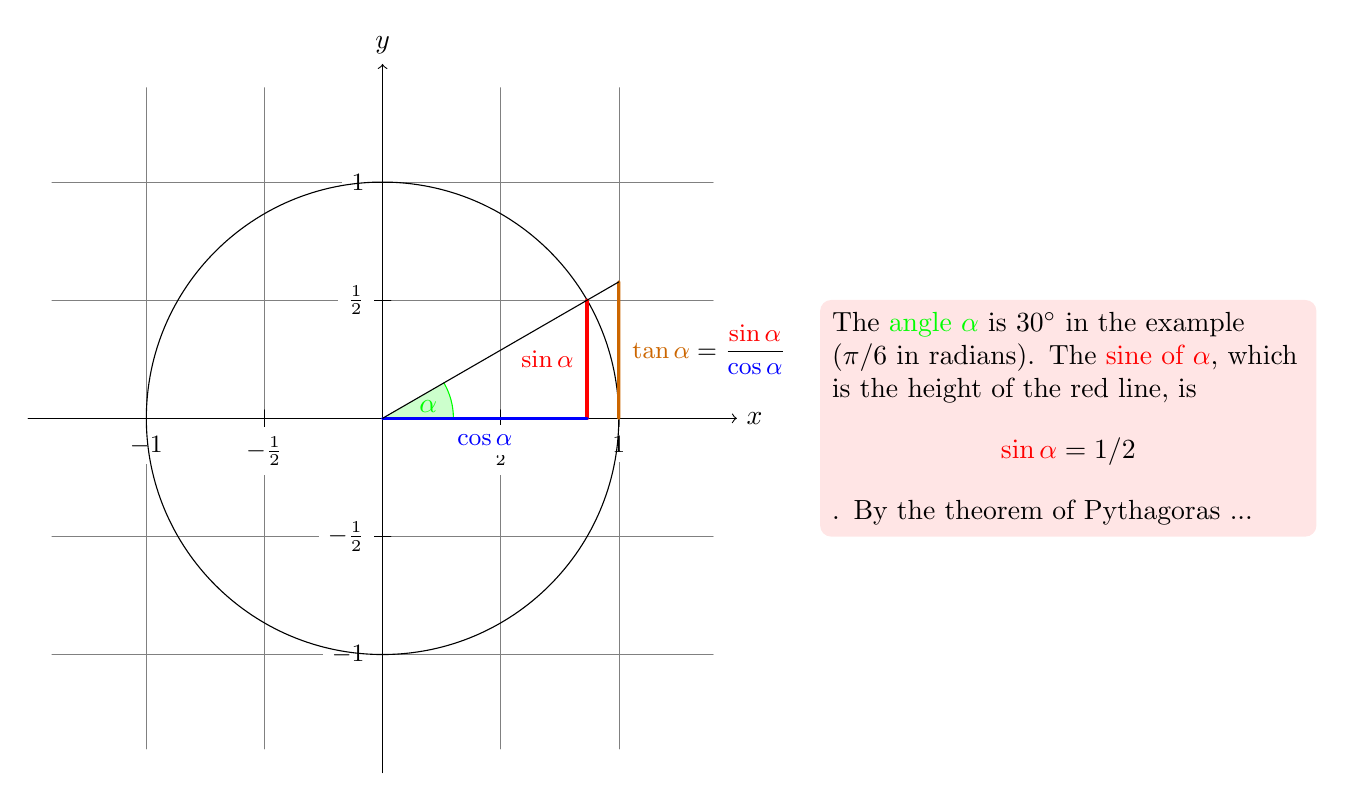
\begin{tikzpicture}[scale=3, line cap=round,
		% Styles
		axes/.style=,
		important line/.style={very thick},
		information text/.style={rounded corners, fill=red!10, inner sep=1ex}
		]
		
		% Colors
		\colorlet{anglecolor}{green!150!black}
		\colorlet{sincolor}{red}
		\colorlet{coscolor}{blue}
		\colorlet{tancolor}{orange!80!black}
		
		% \clip[draw] (-1.5, -0.4) rectangle (2.2, 1.52);
		
		% The graphic
		% help lines: provided by tikz package itself
		\draw[help lines, step=0.5cm] (-1.4, -1.4) grid (1.4, 1.4);
		
		\begin{scope}[axes]
			\draw[->] (-1.5, 0) -- (1.5, 0) node[right] {$x$} coordinate(x axis); % x-axis
			\draw[->] (0, -1.5) -- (0, 1.5) node[above] {$y$} coordinate(y axis); % y-axis
			
			\foreach \x/\xtext in {-1, -0.5/-\frac{1}{2}, 0.5/\frac{1}{2}, 1}
				\draw[xshift=\x cm] (0pt, 1pt) -- (0pt, -1pt) node[below, fill=white] {\small $\xtext$};
			\foreach \y/\ytext in {-1, -0.5/-\frac{1}{2}, 0.5/\frac{1}{2}, 1}
			\draw[yshift=\y cm] (1pt, 0pt) -- (-1pt, 0pt) node[left, fill=white] {\small $\ytext$};
		\end{scope}
		
		
		\draw (0, 0) circle [radius=1cm];
		
		% Angle
		\filldraw[fill=green!20, draw=anglecolor] (0, 0) -- (3mm, 0pt)
		arc [start angle=0, end angle=30, radius=3mm];
		\draw (15:2mm) node[anglecolor] {$\alpha$};
		
		% Sine line
		\draw[important line, sincolor] (30:1cm) -- node [left=1pt, fill=white] {\small $\sin \alpha$} (30:1cm |- x axis);  % |- is the point at intersection.
		% Cosine line
		\draw[important line, coscolor] (30:1cm |- x axis) -- node [below=2pt, fill=white] {\small $\cos \alpha$} (0, 0);
		
		% \path without draw or fill option is not displayed.
		\path [name path=upward line] (1, 0) -- (1,1);
		\path [name path=sloped line] (0, 0) -- (30:1.5cm);    % a bit longer, so that there is an intersection
		
		% Tan line
		% (add `\usetikzlibrary{intersections}` after loading tikz in the preamble)
		\draw [name intersections={of=upward line and sloped line, by=newCoordinates}]
			[important line, tancolor] (1, 0) -- node [right=1pt, fill=white] {\small $\displaystyle \tan \alpha \color{black} = \frac{\color{red}\sin \alpha}{\color{blue}\cos \alpha}$} (newCoordinates);
			
		% Line from origin to tan line
		\draw (0, 0) -- (newCoordinates);
		
		\draw[xshift=1.85cm] 
			node[information text, text width=6cm, right] {
				The {\color{anglecolor} angle $\alpha$} is $30^\circ$ in the example ($\pi/6$ in radians). The {\color{sincolor}sine of $\alpha$}, which is the height of the red line, is 
				\[
					{\color{sincolor}\sin \alpha} = 1/2
				\]
				. By the theorem of Pythagoras ...
			};
		
	\end{tikzpicture}
\end{document}